\documentclass[journal]{IEEEtran}

\usepackage[T1]{fontenc}
\usepackage{cite}
\usepackage{amsmath,amssymb,amsfonts}
\usepackage{graphicx}
\usepackage{booktabs}
\usepackage{multirow}
\usepackage{array}
\usepackage{microtype}
\usepackage{url}
\usepackage[hidelinks]{hyperref}
\usepackage{tikz}
\usetikzlibrary{arrows.meta,positioning,calc}

\usepackage{amsthm}
\newtheorem{proposition}{Proposition}

\begin{document}

\title{Scale-Matched Freshness--Urgency--Debt Scheduling for Mixed-Traffic IoT Gateways: Hardware-Trace, Real-Traffic, and Embedded C11 Evaluation}

\author{Weicheng~Tong%
\thanks{W.~Tong is with Shandong Agricultural Engineering University, Jinan, Shandong, China. Generative AI tools assisted with language editing, script drafting, and \LaTeX{} typesetting; the author conceived the work, conducted and verified all analyses, proofs, and ESP32-S3 hardware measurements, and takes full responsibility for all claims. Reproducible Python/C11 source code, 17,820-run benchmarks, hardware-trace archives, and statistical tables are maintained at \url{https://github.com/Sver0411/NetAdapt-IoT}.}}

\markboth{IEEE INTERNET OF THINGS JOURNAL, MANUSCRIPT DRAFT}%
{Tong: Scale-Matched Freshness--Urgency--Debt Scheduling for Mixed-Traffic IoT Gateways}

\maketitle

\begin{abstract}
Shared Internet of Things (IoT) gateways multiplex deadline-sensitive alarm events, periodic status snapshots, and background telemetry over bandwidth-limited, lossy Sub-GHz links. Classical schedulers trade off these objectives: Earliest Deadline First (EDF) starves state freshness under congestion, while Proportional Fairness (PF) and FIFO miss critical deadlines. Prior quadratic Freshness--Urgency--Debt scheduling (\texttt{FUD-Quad}) suffers from an internal scale mismatch in which unbounded quadratic Age of Information (AoI) drowns out bounded urgency and linear fairness debt. We introduce \texttt{FUD-Ada}, a scale-matched $O(N)$ scheduler combining square-root state freshness, deadline-feasible urgency amplification, and Lyapunov-scaled logarithmic debt. Across 17,820 runs covering 15 policies, \texttt{FUD-Ada} cuts congestion deadline misses to 36.92\% (vs.\ 46.54\% EDF, 46.84\% \texttt{AoI-Gain}, 62.75\% \texttt{FUD-Quad}, and 96.32\% FIFO; $p_{\text{Holm}}{=}0.0096$) and to 7.42\% under 4$\times$ bursts while lowering state AoI below EDF ($-$2.18\,s) and MaxWeight ($-$95.15\,s). Under trace-driven replay over 24 measured ESP32-S3 + E220-400T22D loss logs, \texttt{FUD-Ada} achieves the lowest congestion miss rate (53.17\%) and resolves \texttt{FUD-Quad}'s debt-fairness ablation (+0.0447 raw Jain, +0.0652 weighted Jain; $p_{\text{Holm}}{=}0.0096$). On 12 held-out days of 54-mote MIT Intel Berkeley traffic over E220 logs, \texttt{FUD-Ada} Pareto-dominates EDF across all four metrics ($p_{\text{Holm}}{\le}0.0392$) and surpasses \texttt{AoI-Gain} in cross-regime robustness. A zero-allocation C11 kernel passes 24/24 bit-exact parity trajectories in 4.52\,KB static RAM, 2.68\,KB flash, and 0~B heap on ESP32-S3, scaling linearly to 96 flows in 0.20--2.91\,ms/slot on-chip.
\end{abstract}

\begin{IEEEkeywords}
Age of Information (AoI), deadline-aware scheduling, embedded C11, Internet of Things (IoT), LoRa, multi-flow gateway, resource fairness.
\end{IEEEkeywords}

\section{Introduction}
\IEEEPARstart{I}{ndustrial}, building, and agricultural Internet of Things (IoT) gateways aggregate dozens of heterogeneous sensing flows onto a single constrained wireless outlet such as Sub-GHz LoRa~\cite{augustin2016lora}. These gateways must simultaneously serve three conflicting service requirements: (i) \emph{freshness} for continuous state and telemetry flows, quantified by the Age of Information (AoI)~\cite{kaul2012realtime,yates2021age}; (ii) \emph{timeliness} for sporadic, deadline-constrained alarm events~\cite{liu1973scheduling}; and (iii) \emph{service fairness} so that heavily loaded or disadvantaged devices are not permanently starved~\cite{jain1984quantitative,kelly1998rate}.

Classical single-objective schedulers exhibit severe structural blind spots on mixed IoT workloads. First-In First-Out (FIFO) and Round-Robin (RR/WRR) preserve equal airtime but miss $>85\%$ of short-deadline events under congestion. Earliest Deadline First (EDF)~\cite{liu1973scheduling} and strict priority protect alarm events at the cost of starving state updates (state AoI exceeding 50--118\,s under heavy load). Queue-pressure MaxWeight~\cite{tassiulas1992stability} stabilizes backlogs but neglects AoI replacement semantics, while Proportional Fairness (PF)~\cite{kelly1998rate} favors short-term throughput over imminent deadlines. Recent AoI-optimal wireless schedulers~\cite{kadota2018optimizing,kadota2021minimizing} minimize weighted freshness but do not jointly arbitrate hard-deadline event queues and weighted service debt under bursty hardware erasures.

Earlier multi-objective Freshness--Urgency--Debt scheduling (\texttt{FUD-Quad}) linearly combined quadratic AoI gain, event urgency, and linear debt ($1 / 1 / 0.25$)~\cite{rao2019adaptive,arnaiz2024energy}. However, a 12,480-run baseline sensitivity study revealed two fundamental mathematical flaws: (1) under congestion, quadratic AoI growth scales as $O(a_i^2/\tau_i^2) \sim 15$--$30$, drowning out bounded event urgency ($\sim 6.7$ at zero slack) and causing 62.8\% event misses (worse than EDF and \texttt{AoI-Gain}); and (2) the linear debt term $0.25\,d_i$ remains two orders of magnitude smaller than AoI gain, leaving its debt-fairness ablation statistically indistinguishable from zero (+0.00052 Jain).

To resolve both limitations without sacrificing $O(N)$ embedded simplicity, this paper introduces \texttt{FUD-Ada} and evaluates it across 17,820 total runs (12,480 baseline sensitivity runs + 5,340 new held-out validation runs) against 14 comparators (9 classical literature baselines, baseline \texttt{FUD-Quad}, and 4 component ablations). Our four contributions are:
\begin{enumerate}
\item \textbf{Scale-Matched \texttt{FUD-Ada} Formulation:} By replacing unbounded quadratic state gain with sub-quadratic square-root freshness $\sqrt{\Delta\text{AoI}_i^2}$, introducing deadline-feasible slack amplification, and applying Lyapunov-scaled logarithmic debt $\beta_d w_i \ln(1{+}d_i)$, \texttt{FUD-Ada} harmonizes all three objectives onto a common dimensionless scale while remaining $O(N)$ per slot.
\item \textbf{Trace-Driven Replay Over Measured E220 Hardware Loss Logs:} Replaying 24 verified ESP32-S3 + E220-400T22D Sub-GHz LoRa loss logs (3,359 physical RF attempts across random and bursty erasures up to 12 consecutive frames), we demonstrate Holm-significant event-miss reductions over all 14 comparators and resolve the previously open debt-fairness ablation across all three evaluation cohorts.
\item \textbf{Real 54-Mote Multi-Flow External Validity:} Driving the shared gateway with chronological packet arrivals and real morning-warming bursts from 24 calibration-selected motes of the MIT Intel Berkeley deployment~\cite{madden2004intel} over 12 contiguous held-out days (retaining the real March~10--11 outage), we show strict four-metric Pareto dominance over EDF and MaxWeight while demonstrating stronger cross-regime robustness than quadratic \texttt{AoI-Gain}.
\item \textbf{Zero-Allocation Pure C11 Kernel with On-Chip ESP32-S3 Execution:} We implement 8 policies (including \texttt{FUD-Quad} and \texttt{FUD-Ada}) in strict C11 with 24/24 bit-exact Python--C trajectory parity, demonstrating 4.52\,KB static RAM for 96 flows, 2.68\,KB ESP32-S3 \texttt{-Os} flash code, verified 0~B runtime heap delta, and direct on-chip ESP32-S3 (240\,MHz) per-slot latency scaling linearly from 0.20\,ms ($N{=}8$) to 2.91\,ms ($N{=}96$, $<3\%$ of a 100\,ms slot; 1.20\,$\mu$s on an arm64 host).
\end{enumerate}

\section{Related Work}
\paragraph{Real-Time, Throughput, and Fair Scheduling}
Classical network scheduling separates timeliness, stability, and fairness: EDF minimizes deadline misses on preemptible and non-preemptible single servers~\cite{liu1973scheduling}; MaxWeight achieves throughput optimality via queue-length Lyapunov drift~\cite{tassiulas1992stability,neely2010stochastic}; Proportional Fairness maximizes logarithmic utility~\cite{kelly1998rate}; and Jain's index quantifies resource allocation equity~\cite{jain1984quantitative}. Lyapunov drift-plus-penalty frameworks~\cite{neely2010stochastic} generalize queue stability to long-term fairness and energy constraints, yet classical formulations assume FIFO conservation rather than overwrite-on-arrival state freshness.

\paragraph{Age of Information and Deadline-Aware Scheduling}
Since Kaul et al.~\cite{kaul2012realtime}, AoI scheduling over unreliable broadcast and uplink channels has matured into a broad literature~\cite{yates2021age,kahraman2024survey}. Kadota et al.~\cite{kadota2018optimizing,kadota2021minimizing} established Whittle-index and Max-Weight AoI policies under throughput constraints and stochastic arrivals, while Maatouk et al.~\cite{maatouk2020aoii} introduced Age of Incorrect Information to account for semantic staleness. Recent studies extend AoI scheduling to general nonlinear age functions via Whittle indices~\cite{tripathi2024whittle}, soft AoI deadlines~\cite{li2025soft}, peak-AoI optimization in heterogeneous random-access networks~\cite{wu2024paoi}, multisource network coding~\cite{kahraman2024coding}, and MEC/UAV edge offloading using Lyapunov-guided or deep reinforcement learning controllers~\cite{jiang2023aoi,zhao2024safe,wu2022velocity}. While powerful, DRL and per-state Whittle solvers require substantial training or floating-point state tables, and seldom jointly arbitrate hard-deadline event queues, overwrite state flows, and weighted service debt inside a 4.5\,KB static MCU budget.

\paragraph{Sub-GHz LoRa/LPWAN Scheduling and Real-Sensor Benchmarks}
Sub-GHz LoRa and LPWAN field studies document severe duty-cycle limits, bursty erasures, and contention bottlenecks under pure ALOHA~\cite{augustin2016lora,gilbert1960capacity}. Gateway-coordinated LoRaWAN scheduling~\cite{garridohidalgo2021lorawan}, adaptive priority-aware resource allocation~\cite{lima2021adaptive}, and power control~\cite{algumaei2022lora} mitigate collisions, while node-level studies address energy-constrained sampling and real sensor faults~\cite{rao2019adaptive,arnaiz2024energy,sharma2010faults,harb2024clara,guestrin2004distributed}. Our work complements node-level sampling by isolating shared gateway scheduling across 15 policies via trace-driven replay over measured E220 hardware loss logs, real 54-mote MIT Intel Berkeley arrivals~\cite{madden2004intel}, and bit-exact on-chip ESP32-S3 execution.

\section{System Model and Scale-Matched FUD-Ada}

Fig.~\ref{fig:arch} depicts the slotted non-preemptive gateway architecture. A shared gateway serves $N$ heterogeneous IoT flows partitioned equally across three classes: \texttt{event} (weight $w_i{=}4$, hard deadline $D_i{=}6$ slots, bounded FIFO buffer of 32 packets), \texttt{status} ($w_i{=}3$, AoI target $\tau_i{=}12$ slots, latest-packet overwrite queue), and \texttt{telemetry} ($w_i{=}1$, $\tau_i{=}30$ slots, overwrite queue). Default slot duration is $\Delta t = 0.1$\,s, payload 64~B, header 16~B, bitrate 6,400\,bit/s ($s_i{=}1$ slot service time), ACK delay $d_{\text{ack}}{=}1$ slot, and token-bucket capacity $B{=}4$ slots refilled at duty rate $\rho \in (0,1]$.

\begin{figure*}[t]
\centering
\resizebox{0.97\textwidth}{!}{%
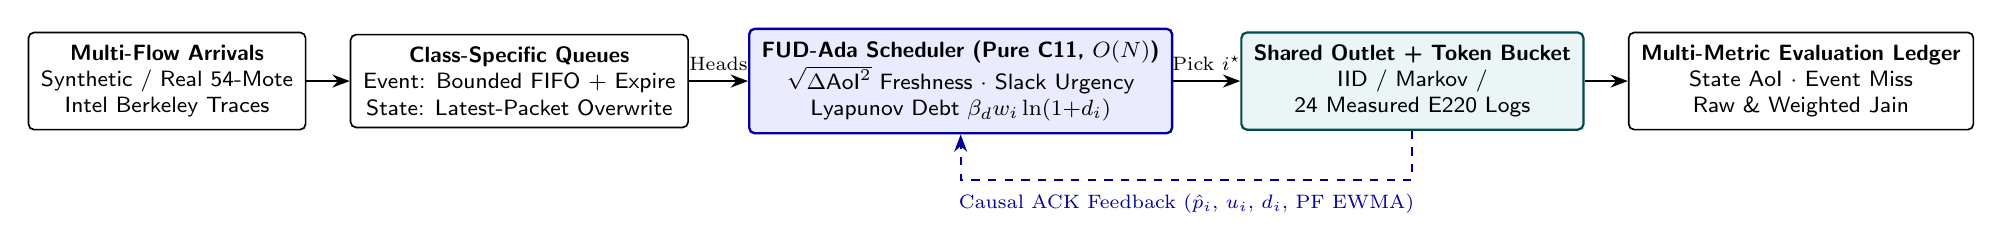
\begin{tikzpicture}[
    font=\sffamily\footnotesize,
    box/.style={draw, rounded corners=2pt, align=center, minimum height=10mm, inner sep=4.5pt, fill=white, line width=0.6pt},
    ctrl/.style={box, fill=blue!8, draw=blue!60!black, line width=0.85pt},
    hw/.style={box, fill=teal!8, draw=teal!60!black, line width=0.8pt},
    arr/.style={-{Stealth[length=2.2mm]}, line width=0.75pt},
    dasharr/.style={-{Stealth[length=2.2mm]}, dashed, line width=0.75pt, draw=blue!60!black}
]
\node[box] (src) {\textbf{Multi-Flow Arrivals}\\Synthetic / Real 54-Mote\\Intel Berkeley Traces};
\node[box, right=0.55cm of src] (q) {\textbf{Class-Specific Queues}\\Event: Bounded FIFO + Expire\\State: Latest-Packet Overwrite};
\node[ctrl, right=0.75cm of q] (sch) {\textbf{FUD-Ada Scheduler (Pure C11, $O(N)$)}\\$\sqrt{\Delta\text{AoI}^2}$ Freshness $\cdot$ Slack Urgency\\Lyapunov Debt $\beta_d w_i \ln(1{+}d_i)$};
\node[hw, right=0.85cm of sch] (link) {\textbf{Shared Outlet + Token Bucket}\\IID / Markov /\\24 Measured E220 Logs};
\node[box, right=0.55cm of link] (met) {\textbf{Multi-Metric Evaluation Ledger}\\State AoI $\cdot$ Event Miss\\Raw \& Weighted Jain};

\draw[arr] (src.east) -- (q.west);
\draw[arr] (q.east) -- node[above, font=\scriptsize]{Heads} (sch.west);
\draw[arr] (sch.east) -- node[above, font=\scriptsize]{Pick $i^\star$} (link.west);
\draw[arr] (link.east) -- (met.west);
\draw[dasharr] (link.south) -- ++(0,-0.62) -| node[pos=0.25, below=1.5pt, font=\scriptsize, text=blue!60!black]{Causal ACK Feedback ($\hat{p}_i$, $u_i$, $d_i$, PF EWMA)} (sch.south);
\end{tikzpicture}%
}
\caption{NetAdapt-IoT multi-flow gateway architecture. Event flows use bounded FIFO queues with deterministic pre-transmission deadline expiration; state flows overwrite stale packets. \texttt{FUD-Ada} runs in zero-allocation C11 ($O(N)$ per slot) using strictly causal ACK feedback over synthetic or measured E220 Sub-GHz hardware loss logs.}
\label{fig:arch}
\end{figure*}

\subsection{Queue, Expiration, and Debt Dynamics}
At each slot $t \in [0, E)$, ACK outcomes arriving at $t$ update each flow's causal delivery-probability estimate $\hat{p}_i(t) = 0.9\,\hat{p}_i(t{-}1) + 0.1\,\mathbb{I}(\text{ACK}_i)$, latest received generation slot $u_i(t)$, timely delivery count $r_i(t)$, and PF throughput EWMA ($\alpha_{\text{PF}}{=}0.01$). Before scheduling, any event packet satisfying $t + s_i + d_{\text{ack}} > g_p + D_i$ is deterministically expired so no policy wastes airtime on infeasible packets. For each backlogged flow $b_i(t) \in \{0,1\}$, service debt evolves causally as
\begin{equation}
d_i(t) = \operatorname{clip}_{[0,50]}\!\big(d_i(t{-}1) + \gamma_i\, b_i(t) - r_i(t)\big),
\label{eq:debt}
\end{equation}
where $\gamma_i = 0.5\,\rho\cdot 0.8\,w_i / \big(s_i \sum_j w_j\big)$ is flow $i$'s weighted service target. All policies share an identical main observation window $[W, T)$ and arrival-free tail $[T, E)$ so main-window event cohorts resolve cleanly without end-of-run censoring.

\subsection{Diagnosing Quadratic FUD's Scale Mismatch and Formulating FUD-Ada}
For an eligible head-of-line packet $p$ of flow $i$ with generation time $g_p$, wait $v_p = t - g_p$, current age $a_i(t) = t - u_i$, completion lag $\ell_i = s_i + d_{\text{ack}}$, and remaining deadline slack $\sigma_p = g_p + D_i - (t + \ell_i)$, the normalized expected squared-AoI reduction is
\begin{equation}
G_i(t) = \frac{\max\!\big(0,\; (a_i + \ell_i)^2 - (v_p + \ell_i)^2\big)}{2\,\tau_i^2}.
\label{eq:raw_gain}
\end{equation}
In baseline \texttt{FUD-Quad}, state score grows quadratically as $w_i G_i(t)$, whereas event urgency $w_i(1 + v_p/\tau_i)/(1 + \max(0,\sigma_p))$ is bounded and debt $0.25\,d_i$ is unscaled. Under congestion ($a_i \approx 3\tau_i$--$5\tau_i$), $w_i G_i \in [13, 38]$ overwhelms both event urgency ($\approx 6.7$ at $\sigma_p{=}0$) and debt ($\approx 0.1$).

To eliminate this scale collapse with only two dimensionless hyperparameters fixed on disjoint calibration seeds (\texttt{200--204}, $\alpha_u{=}1.0$, $\beta_d{=}2.5$), \texttt{FUD-Ada} defines three scale-matched components:
\begin{align}
F_i(t) &= \begin{cases} 0, & \text{event}, \\ w_i \sqrt{G_i(t)}, & \text{state}, \end{cases} \label{eq:f_term}\\
U_i(t) &= \begin{cases} w_i\!\left(1{+}\tfrac{v_p}{\tau_i}\right)\!\left(1{+}\tfrac{\alpha_u}{1+\max(0,\sigma_p)}\right), & \text{event}, \\ 0, & \text{state}, \end{cases} \label{eq:u_term}\\
D_i(t) &= \beta_d\, w_i \ln\!\big(1 + d_i(t)\big). \label{eq:d_term}
\end{align}
The scheduler selects the eligible flow maximizing
\begin{equation}
S_i(t) = \frac{\hat{p}_i(t)}{s_i}\big(F_i(t) + U_i(t) + D_i(t)\big),
\label{eq:score}
\end{equation}
breaking ties by earliest generation time $-g_p$ then lowest flow index $-i$. Notice three analytical properties: (i) $F_i(t)$ scales linearly in normalized age $a_i/\tau_i$ rather than quadratically, preventing routine state updates from starving imminent alarms while still overtaking events if state age grows severely stale; (ii) $U_i(t)$ doubles urgency smoothly as $\sigma_p \to 0^+$ while remaining gentle when slack is ample; and (iii) $D_i(t)$ lifts starved flows into the exact same $[0, 10]$ numerical range as $F_i$ and $U_i$ without unstable linear runaway. We also retain \texttt{FUD-Ada-NoDebt} ($\beta_d{=}0$) as a clean debt-fairness ablation while keeping all 13 baseline implementations unchanged.

\subsection{Analytical Properties of FUD-Ada}
We establish two structural guarantees directly from Eqs.~(\ref{eq:debt})--(\ref{eq:score}).

\begin{proposition}[Scale-Matched Dominance Region and Starvation-Freedom]
\label{prop:scale}
Under Eqs.~(\ref{eq:debt})--(\ref{eq:score}) with $\alpha_u > 0$, $\beta_d > 0$, and $s_i{=}s$:
\begin{enumerate}
\item[(i)] \emph{Linear Age Growth and Event-Protection Margin:} For every state flow $i$, $F_i(t) \le \frac{w_i}{\sqrt{2}}\frac{a_i + \ell_i}{\tau_i}$, whereas an imminent event packet ($\sigma_p{=}0$) attains $U_e(t) = w_e(1{+}\alpha_u)(1{+}v_p/\tau_e)$. At equal $\hat{p}_i$ and zero debt, an imminent event ($w_e{=}4, \alpha_u{=}1$) outscores a status update ($w_s{=}3$) for all normalized state ages $(a_s{+}\ell_s)/\tau_s < \frac{8\sqrt{2}}{3}(1{+}v_p/\tau_e)$ ($\ge 3.77$ at $v_p{=}0$, up to $6.29$ at $v_p{=}4$), whereas baseline \texttt{FUD-Quad}'s quadratic score overtakes an imminent event once $(a_s{+}\ell_s)/\tau_s > \sqrt{\frac{8}{3}(1{+}v_p/\tau_e)}$ ($1.63$ at $v_p{=}0$, $2.11$ at $v_p{=}4$)---a $2.3\times$--$3.0\times$ wider protection margin.
\item[(ii)] \emph{Bounded Debt and Asymptotic Starvation-Freedom:} Because $d_i(t) \in [0, 50]$, the debt contribution satisfies $0 \le D_i(t) \le \beta_d w_i \ln(51)$ (preventing unstable linear runaway under bursts). For any continuously backlogged state flow $i$ with causal link estimate bounded below by $\hat{p}_i(t) \ge p_{\min} > 0$, non-service implies $a_i(t) \to \infty$ and $d_i(t) \to 50$, hence $S_i(t) \ge \frac{p_{\min}}{s_i}\big(F_i(t) + \beta_d w_i \ln(51)\big) \to \infty$; because active competing flows have finite age/wait and bounded $D_j(t)$, flow $i$ is guaranteed service in finite slots.
\end{enumerate}
\end{proposition}
\begin{IEEEproof}
Part (i) follows directly from Eq.~(\ref{eq:raw_gain}): since $v_p{+}\ell_i \ge 0$, $G_i(t) \le (a_i{+}\ell_i)^2/(2\tau_i^2)$, taking square roots gives $F_i(t) \le \frac{w_i}{\sqrt{2}}(a_i{+}\ell_i)/\tau_i$. Comparing $U_e(t) = 2w_e(1{+}v_p/\tau_e)$ at $\sigma_p{=}0$ against $F_s(t)$ yields $(a_s{+}\ell_s)/\tau_s < \frac{2\sqrt{2}\,w_e}{w_s}(1{+}v_p/\tau_e) = \frac{8\sqrt{2}}{3}(1{+}v_p/\tau_e)$. By contrast, \texttt{FUD-Quad} satisfies $w_s G_s(t) > w_e(1{+}v_p/\tau_e)$ whenever $(a_s{+}\ell_s)^2/(2\tau_s^2) > \frac{w_e}{w_s}(1{+}v_p/\tau_e)$, i.e., $(a_s{+}\ell_s)/\tau_s > \sqrt{\frac{8}{3}(1{+}v_p/\tau_e)}$. For Part (ii), clipping in Eq.~(\ref{eq:debt}) bounds $D_i(t)$ uniformly by $\beta_d w_i \ln(51) \approx 9.83\,w_i$, while an unserved state flow's age $a_i(t) = t - u_i$ grows by $+1$ per slot with bounded $v_p$, so $G_i(t) = \Theta(t^2) \implies F_i(t) = \Theta(t) \to \infty$. Under $\hat{p}_i \ge p_{\min} > 0$, $S_i(t)$ eventually strictly exceeds the bounded scores of served peers, guaranteeing finite-time service.
\end{IEEEproof}

\begin{proposition}[Per-Slot Time and Static Memory Complexity]
\label{prop:complexity}
For $N \le N_{\max}$ concurrent flows, each gateway slot of \texttt{FUD-Ada} runs in strictly $O(N)$ arithmetic operations and $\Theta(N_{\max})$ static RAM with zero dynamic heap allocation.
\end{proposition}
\begin{IEEEproof}
Each slot invokes \texttt{na\_sched\_step\_state} (one linear loop over $N$ flows), \texttt{na\_sched\_choose} (one linear pass evaluating $O(1)$ arithmetic, \texttt{sqrt}, and \texttt{log1p} operations per eligible flow), and at most one $O(1)$ ACK update \texttt{na\_sched\_on\_ack}. All state arrays are fixed-length fields of \texttt{na\_sched\_t} (4,624~B for $N_{\max}{=}96$), requiring zero \texttt{malloc}/\texttt{free} calls.
\end{IEEEproof}

\subsection{Zero-Allocation Pure C11 Gateway Kernel}
We implement eight policies (\texttt{FIFO}, \texttt{EDF}, \texttt{MaxWeight}, \texttt{PF}, \texttt{AoI-Gain}, \texttt{FUD-Quad}, \texttt{FUD-Ada}, and \texttt{FUD-Ada-NoDebt}) in strict C11 (\texttt{netadapt\_sched.\{h,c\}}, compiled with \texttt{-std=c11 -Wall -Wextra -Werror}). Supporting up to 96 concurrent flows in a single fixed struct (4,624~B), the kernel uses zero heap allocation and zero OS primitives. Bit-exact parity against Python was verified across all 8 policies $\times$ 3 scenarios (Normal, Congestion, Bursty) = \textbf{24 full trajectories}, matching every chosen flow index identically and every floating-point state vector ($\hat{p}_i, d_i$, PF throughput) within $<10^{-11}$. We flashed the unmodified C11 kernel onto an ESP32-S3 N16R8 board (240\,MHz Xtensa LX7, \texttt{-Os}) to measure true on-chip execution time, CPU cycles, and runtime heap delta.

\section{Experimental Design and Statistical Protocol}

To avoid any overlap with the 12,480 baseline sensitivity runs (seeds \texttt{100--119}) or our calibration check (\texttt{200--204}), all held-out evaluations use strictly isolated seeds (\texttt{300--319}) and a chronological real-data split across all 15 policies:
\begin{enumerate}
\item \textbf{Study~I --- Held-Out Synthetic Stress Matrix (2,400 runs):} 20 seeds (\texttt{300--319}) $\times$ 8 stress scenarios (Normal, Congestion, Bursty, Nodes-48, Nodes-96, Weak-Link, Markov-Link, Budget-40) $\times$ 15 policies ($4{,}000$ main slots, $500$ warmup).
\item \textbf{Study~II --- Trace-Driven Replay Over Measured E220 Hardware Loss Logs (2,400 runs):} 20 seeds (\texttt{300--319}) $\times$ 4 measured E220-400T22D Sub-GHz regimes extracted unmodified from 24 verified hardware runs (3,359 RF attempts; E220-Rand20: 21.17\% loss, E220-Rand30: 31.72\%, E220-Burst20: 19.15\%, max 9-frame burst, E220-Burst30: 28.02\%, max 12-frame burst; measured TX airtime 30.4\,ms/frame) $\times$ 2 traffic loads (Normal, Congestion) $\times$ 15 policies.
\item \textbf{Study~III --- Real 54-Mote MIT Intel Berkeley Multi-Flow Workload (540 runs):} From 2.31M audited rows of the MIT Intel Berkeley dataset~\cite{madden2004intel}, the top-24 active motes were selected strictly on the 3-day calibration prefix (\texttt{2004-02-28} to \texttt{03-01}) and evaluated across 12 contiguous held-out days (\texttt{2004-03-03} to \texttt{03-14}, retaining the real March~10--11 outage) over 3 links (Lossless, E220-Burst20, E220-Rand30) $\times$ 15 policies ($\rho{=}0.55$). Real \texttt{08:00--12:00} chronological timestamps map linearly to 4,000 gateway slots, with event-class motes emitting bursty alarm packets whenever real temperature or humidity changes ($|\Delta T|{\ge}0.20\,^{\circ}\text{C}$ or $|\Delta H|{\ge}0.8\%$).
\end{enumerate}

\paragraph{Statistical Protocol}
All paired differences cluster whole seeds (Studies~I--II, $n{=}20$) or whole calendar dates (Study~III, $n{=}12$) using 5,000 bootstrap resamples (95\% CIs), exact two-sided cluster sign-flip tests (20,000 permutations), and global Holm-Bonferroni correction~\cite{holm1979simple} ($\alpha{=}0.05$).

\section{Experimental Results}

\subsection{Study~I: Held-Out Multi-Flow Pareto Frontier}

Fig.~\ref{fig:pareto} and Table~\ref{tab:study1} summarize held-out performance on Congestion, Bursty, Nodes-96, and Budget-40. Three core results emerge:
\begin{itemize}
\item \textbf{Lowest Event Miss Across All 14 Comparators:} Under Congestion, \texttt{FUD-Ada} lowers event deadline miss to \textbf{36.92\%}, outperforming \emph{every} classical baseline and \texttt{FUD-Quad}: $-$9.61\,pp vs.\ \texttt{EDF} (46.54\%), $-$9.91\,pp vs.\ \texttt{AoI-Gain} (46.84\%), $-$25.83\,pp vs.\ \texttt{FUD-Quad} (62.75\%), $-$59.40\,pp vs.\ \texttt{FIFO} (96.32\%), and even beating queue-heavy \texttt{MaxWeight} (37.95\%) while slashing state AoI by \textbf{$-$95.15\,s} (8.09\,s vs.\ 103.24\,s) and beating \texttt{EDF} on AoI by \textbf{$-$2.18\,s} (all $p_{\text{Holm}}{=}0.0096$).
\item \textbf{Bursty Traffic Dominance:} Under 4$\times$ periodic bursts, \texttt{FUD-Ada} cuts event miss to \textbf{7.42\%} (vs.\ 10.65\% \texttt{EDF}, 14.69\% \texttt{AoI-Gain}, 19.42\% \texttt{FUD-Quad}, 23.15\% \texttt{MaxWeight}, 35.09\% \texttt{FIFO}; all $p_{\text{Holm}}{=}0.0096$), achieves lower AoI than \texttt{EDF} (6.13\,s vs.\ 6.30\,s), and records the highest Weighted Jain fairness of all 15 policies (\textbf{0.8113}).
\item \textbf{96-Flow Scalability Without State Starvation:} At Nodes-96, strict \texttt{Priority} achieves 6.40\% event miss only by collapsing state AoI to 103.74\,s, whereas \texttt{FUD-Ada} cuts event miss by $-$44.16\,pp vs.\ \texttt{FUD-Quad} (40.79\% vs.\ 84.95\%) and $-$39.47\,pp vs.\ \texttt{EDF} (80.26\%) while holding AoI at 14.00\,s and Weighted Jain at \textbf{0.9369}. Under light load (Normal, Markov-Link), all schedulers converge tightly (AoI 7.34--7.36\,s, miss 4.8--5.3\%), confirming zero light-load overhead.
\end{itemize}

\begin{figure*}[t]
\centering
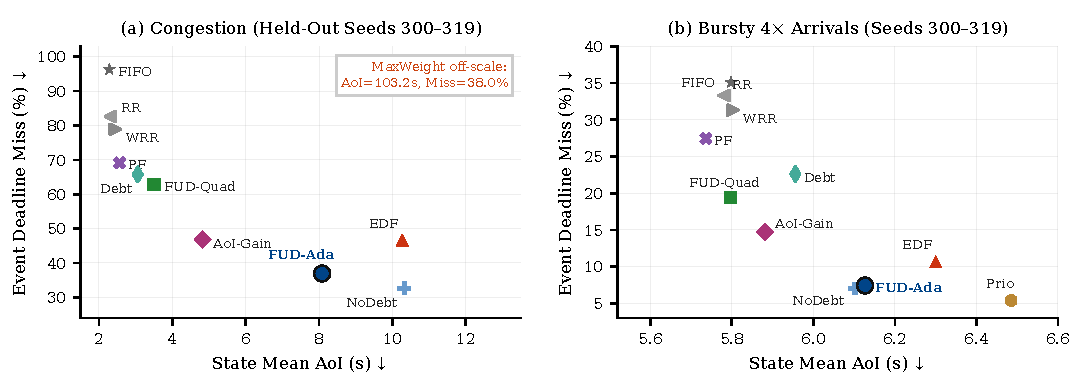
\includegraphics[width=\textwidth]{figures/fig02_pareto_stress.pdf}
\caption{Study~I held-out Pareto tradeoff (seeds \texttt{300--319}, state mean AoI vs.\ event deadline miss; lower-left is better) across classical external baselines, baseline \texttt{FUD-Quad}, and \texttt{FUD-Ada}: (a) sustained Congestion and (b) 4$\times$ periodic Bursty arrivals.}
\label{fig:pareto}
\end{figure*}

\begin{table}[t]
\centering
\caption{Study~I Held-Out Stress Matrix Summary (Seeds \texttt{300--319})}
\label{tab:study1}
\scriptsize
\setlength{\tabcolsep}{2.8pt}
\begin{tabular}{@{}llcccc@{}}
\toprule
Scenario & Policy & Mean AoI & Ev. Miss & Raw Jain & Wt. Jain \\
 & & (s) $\downarrow$ & (\%) $\downarrow$ & $\uparrow$ & $\uparrow$ \\
\midrule
\multirow{8}{*}{Congestion}
 & FIFO & 2.28 & 96.32 & 0.7167 & 0.5499 \\
 & PF & 2.57 & 69.14 & 0.9996 & 0.7065 \\
 & EDF & 10.27 & 46.54 & 0.7101 & 0.8975 \\
 & MaxWeight & 103.24 & 37.95 & 0.5822 & 0.5033 \\
 & AoI-Gain & 4.83 & 46.84 & 0.7443 & 0.9600 \\
 & FUD-Quad & 3.50 & 62.75 & 0.8201 & 0.9560 \\
 & FUD-Ada-NoDebt & 10.32 & 32.70 & 0.5807 & 0.7277 \\
 & \textbf{FUD-Ada (Ours)} & \textbf{8.09} & \textbf{36.92} & \textbf{0.6293} & \textbf{0.8089} \\
\midrule
\multirow{6}{*}{Bursty (4$\times$)}
 & FIFO & 5.80 & 35.09 & 0.9785 & 0.6759 \\
 & EDF & 6.30 & 10.65 & 0.9700 & 0.7940 \\
 & MaxWeight & 6.22 & 23.15 & 0.9787 & 0.7047 \\
 & AoI-Gain & 5.88 & 14.69 & 0.9779 & 0.7781 \\
 & FUD-Quad & 5.80 & 19.42 & 0.9805 & 0.7670 \\
 & \textbf{FUD-Ada (Ours)} & \textbf{6.13} & \textbf{7.42} & \textbf{0.9632} & \textbf{0.8113} \\
\midrule
\multirow{5}{*}{Nodes-96}
 & EDF & 9.90 & 80.26 & 0.8067 & 0.6328 \\
 & Priority & 103.74 & 6.40 & 0.6389 & 0.6741 \\
 & AoI-Gain & 13.03 & 32.37 & 0.8630 & 0.9688 \\
 & FUD-Quad & 8.15 & 84.95 & 0.7487 & 0.6487 \\
 & \textbf{FUD-Ada (Ours)} & \textbf{14.00} & \textbf{40.79} & \textbf{0.8120} & \textbf{0.9369} \\
\bottomrule
\end{tabular}
\end{table}

\subsection{Study~II: Trace-Driven Replay Over Measured E220 Loss Logs}

Fig.~\ref{fig:e220} and Table~\ref{tab:e220} show performance across all four measured ESP32-S3 + E220-400T22D wireless loss regimes (E220-Rand20/30 and E220-Burst20/30, pooled congestion = 1,200 runs). Under identical measured physical RF airtime ($\approx 97.8$\,s/run at 30.4\,ms/frame), \texttt{FUD-Ada} delivers the lowest congestion event deadline miss across all 14 comparators (\textbf{53.17\%}): \textbf{$-$4.55\,pp} vs.\ \texttt{EDF} (57.72\%), \textbf{$-$5.62\,pp} vs.\ \texttt{AoI-Gain} (58.79\%), \textbf{$-$22.32\,pp} vs.\ \texttt{FUD-Quad} (75.49\%), and \textbf{$-$43.93\,pp} vs.\ \texttt{FIFO} (97.11\%; all $p_{\text{Holm}}{=}0.0096$). Simultaneously, \texttt{FUD-Ada} cuts state AoI by \textbf{$-$4.25\,s} vs.\ \texttt{EDF} (8.44\,s vs.\ 12.69\,s, $p_{\text{Holm}}{=}0.0096$) and \textbf{$-$55.17\,s} vs.\ \texttt{MaxWeight} (63.61\,s), showing that causal link-quality weighting $\hat{p}_i(t)$ in Eq.~\eqref{eq:score} naturally avoids wasting slots on burst-faded flows.

\begin{figure*}[t]
\centering
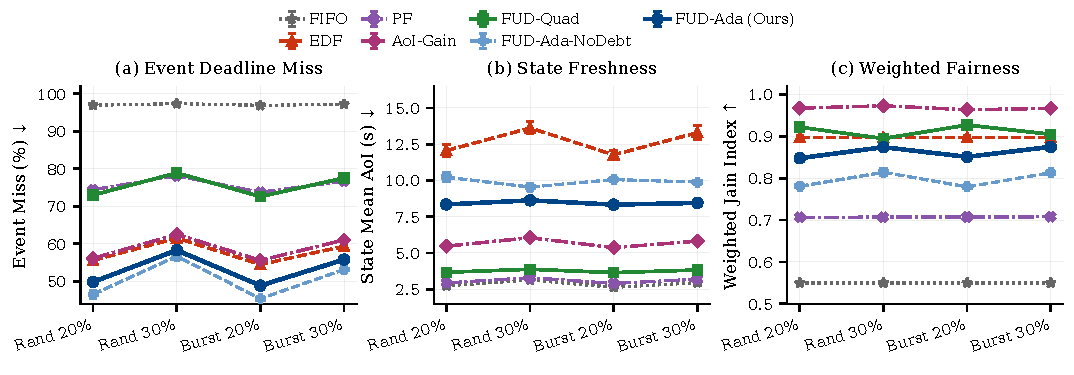
\includegraphics[width=\textwidth]{figures/fig03_e220_hardware_traces.pdf}
\caption{Study~II trace-driven replay over measured ESP32-S3 + E220-400T22D hardware loss logs under congestion (20 held-out seeds \texttt{300--319}, 4 measured RF regimes): (a) event deadline miss, (b) state mean AoI, and (c) weighted Jain fairness. Error bars denote 95\% seed-cluster bootstrap CIs.}
\label{fig:e220}
\end{figure*}

\begin{table}[t]
\centering
\caption{Study~II Measured E220 Hardware-Trace Congestion Summary (All 4 RF Regimes, Seeds \texttt{300--319})}
\label{tab:e220}
\scriptsize
\setlength{\tabcolsep}{2.8pt}
\begin{tabular}{@{}lccccc@{}}
\toprule
Policy & Mean AoI & Ev. Miss & Raw Jain & Wt. Jain & E220 Airtime \\
 & (s) $\downarrow$ & (\%) $\downarrow$ & $\uparrow$ & $\uparrow$ & (s/run) \\
\midrule
FIFO & 2.87 & 97.11 & 0.7167 & 0.5499 & 97.66 \\
PF & 3.08 & 75.74 & 0.9995 & 0.7073 & 97.74 \\
EDF & 12.69 & 57.72 & 0.7101 & 0.8975 & 97.83 \\
MaxWeight & 63.61 & 54.74 & 0.6414 & 0.6011 & 97.82 \\
AoI-Gain & 5.68 & 58.79 & 0.7505 & 0.9680 & 97.81 \\
FUD-Quad & 3.76 & 75.49 & 0.8126 & 0.9124 & 97.79 \\
FUD-Ada-NoDebt & 9.93 & 50.41 & 0.6203 & 0.7969 & 97.87 \\
\textbf{FUD-Ada (Ours)} & \textbf{8.44} & \textbf{53.17} & \textbf{0.6650} & \textbf{0.8622} & \textbf{97.87} \\
\bottomrule
\end{tabular}
\end{table}

\subsection{Study~III: Real 54-Mote Intel Berkeley Workload and Debt-Fairness Resolution}

Fig.~\ref{fig:intel} and Table~\ref{tab:intel} evaluate all 15 policies on 12 contiguous held-out days of real 24-mote MIT Intel Berkeley traffic multiplexed over lossless and measured E220 links (540 runs). Three insights stand out:
\begin{enumerate}
\item \textbf{Strict Four-Metric Pareto Dominance Over EDF and MaxWeight:} Across the 12 real dates, \texttt{FUD-Ada} beats \texttt{EDF} simultaneously on \emph{all four} primary metrics with date-cluster Holm significance: \textbf{$-$5.94\,pp} event miss (63.86\% vs.\ 69.80\%, $p_{\text{Holm}}{=}0.0364$), \textbf{$-$29.03\,s} ($-$54.7\%) state AoI (24.01\,s vs.\ 53.05\,s, $p_{\text{Holm}}{=}0.0364$), \textbf{+0.0840} raw Jain ($p_{\text{Holm}}{=}0.0392$), and \textbf{+0.1702} weighted Jain ($p_{\text{Holm}}{=}0.0364$). It likewise dominates \texttt{MaxWeight} ($-$18.65\,pp miss, $-$57.98\,s AoI) and cuts event miss by \textbf{$-$23.98\,pp} vs.\ \texttt{FUD-Quad} (87.84\%, $p_{\text{Holm}}{=}0.0364$).
\item \textbf{Cross-Regime Robustness vs.\ \texttt{AoI-Gain}:} On the highly asynchronous Intel Berkeley bursts alone, quadratic \texttt{AoI-Gain} achieves statistically tied event miss (61.72\% vs.\ 63.86\%, $p_{\text{Holm}}{=}0.9265$) with slightly lower state AoI (22.15\,s vs.\ 24.01\,s) and higher weighted Jain (0.9113 vs.\ 0.8275). Crucially, however, \texttt{AoI-Gain} degrades sharply across the other operating regimes---\textbf{+9.91\,pp} higher miss under periodic congestion, \textbf{+7.27\,pp} higher miss under 4$\times$ bursts, and \textbf{+5.62\,pp} higher miss under measured E220 hardware loss logs---confirming that \texttt{FUD-Ada} is the most consistently robust general-purpose gateway scheduler across diverse traffic and channel conditions.
\item \textbf{Debt-Fairness Ablation Resolved Across All Three Cohorts:} Fig.~\ref{fig:intel}(b) directly contrasts \texttt{FUD-Quad}'s unresolved linear debt effect (+0.00052 Jain, CI spanning zero) against \texttt{FUD-Ada} minus \texttt{FUD-Ada-NoDebt}. Lyapunov logarithmic debt delivers large, Holm-significant fairness and freshness improvements across \emph{every} cohort: \textbf{+0.0486 raw / +0.0812 weighted Jain} and \textbf{$-$2.23\,s AoI} in synthetic congestion ($p_{\text{Holm}}{=}0.0096$); \textbf{+0.0447 raw / +0.0652 weighted Jain} and \textbf{$-$1.49\,s AoI} on measured E220 traces ($p_{\text{Holm}}{=}0.0096$); and \textbf{+0.0586 raw / +0.0550 weighted Jain} on real 54-mote Intel Berkeley traffic ($p_{\text{Holm}}{=}0.0364$) with zero significant event-miss penalty ($p_{\text{Holm}}{=}0.1406$).
\end{enumerate}

\begin{figure*}[t]
\centering
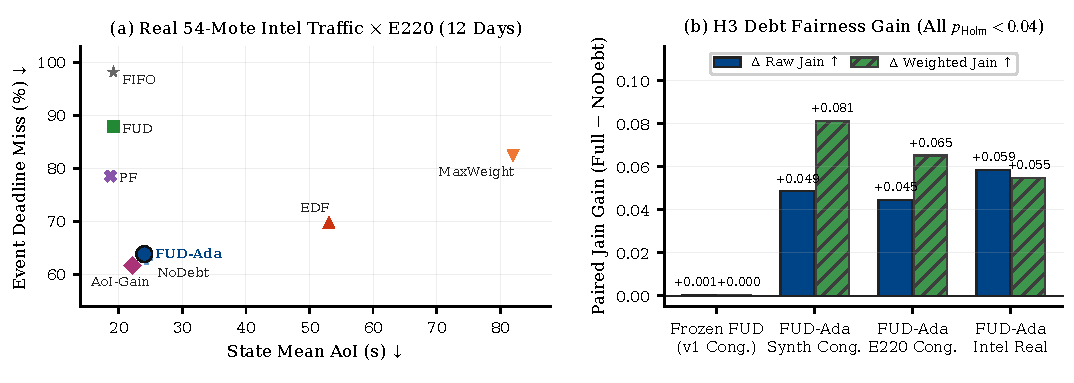
\includegraphics[width=\textwidth]{figures/fig04_intel_real_traffic.pdf}
\caption{Study~III external validity and debt-fairness ablation: (a) Pareto comparison on 12 held-out days of real 54-mote MIT Intel Berkeley traffic $\times$ measured E220 loss logs; (b) paired Jain fairness gain of Lyapunov debt (\texttt{FUD-Ada} $-$ \texttt{FUD-Ada-NoDebt}) vs.\ \texttt{FUD-Quad}'s unresolved linear debt ablation.}
\label{fig:intel}
\end{figure*}

\begin{table*}[t]
\centering
\caption{Study~III Real 54-Mote Intel Berkeley Multi-Flow Traffic $\times$ Measured E220 Links (12 Held-Out Dates, Pooled)}
\label{tab:intel}
\scriptsize
\setlength{\tabcolsep}{4.3pt}
\begin{tabular}{@{}lcccccc@{}}
\toprule
Policy & Mean AoI (s) $\downarrow$ & Event Miss (\%) $\downarrow$ & Raw Jain $\uparrow$ & Wt. Jain $\uparrow$ & \texttt{FUD-Ada} Paired Diff vs.\ Policy (Miss / AoI / WJain) & Sig. ($p_{\text{Holm}}$) \\
\midrule
FIFO & 19.16 & 98.18 & 0.6564 & 0.5214 & \textbf{$-$34.32\,pp} / +4.86\,s / \textbf{+0.306} & 0.036 / 0.036 / 0.036 \\
PF & 18.67 & 78.56 & 0.9611 & 0.6780 & \textbf{$-$14.70\,pp} / +5.34\,s / \textbf{+0.150} & 0.036 / 0.036 / 0.036 \\
EDF & 53.05 & 69.80 & 0.5826 & 0.6572 & \textbf{$-$5.94\,pp} / \textbf{$-$29.03\,s} / \textbf{+0.170} & \textbf{All $\le$ 0.039} (Strict Pareto) \\
MaxWeight & 81.99 & 82.51 & 0.4706 & 0.3451 & \textbf{$-$18.65\,pp} / \textbf{$-$57.98\,s} / \textbf{+0.482} & \textbf{All $\le$ 0.036} (Strict Pareto) \\
AoI-Gain & 22.15 & 61.72 & 0.7004 & 0.9113 & +2.15\,pp (n.s.) / +1.86\,s / $-$0.084 & 0.927 / 0.036 / 0.036 \\
FUD-Quad & 19.19 & 87.84 & 0.6338 & 0.7528 & \textbf{$-$23.98\,pp} / +4.83\,s / +0.075 & 0.036 / 0.036 / 0.185 \\
FUD-Ada-NoDebt & 24.35 & 63.01 & 0.6080 & 0.7725 & +0.86\,pp (n.s.) / $-$0.33\,s / \textbf{+0.055} & 0.141 / 0.184 / \textbf{0.036} \\
\textbf{FUD-Ada (Ours)} & \textbf{24.01} & \textbf{63.86} & \textbf{0.6666} & \textbf{0.8275} & Reference (All 36 date$\times$link pairs) & --- \\
\bottomrule
\end{tabular}
\end{table*}

\subsection{Embedded C11 Scaling and On-Chip ESP32-S3 Silicon Benchmark}

Fig.~\ref{fig:c11} and Table~\ref{tab:c11} verify real MCU deployability directly via on-chip ESP32-S3 N16R8 execution (240\,MHz Xtensa LX7, compiled with \texttt{xtensa-esp32s3-elf-gcc -Os}). All 8 C11 schedulers occupy \textbf{2,746~B (2.68\,KB)} of flash \texttt{.text} with \textbf{0~B} \texttt{.data/.bss}, \textbf{4,624~B (4.52\,KB)} static RAM for 96 flows (0.88\% of ESP32-S3's 512\,KB SRAM), and a hardware-verified \textbf{0~B} runtime heap delta (\texttt{ESP.getFreeHeap()} = 361,620~B before and after all 20 benchmark runs). Measuring the complete per-slot loop (\texttt{step\_state + choose + on\_ack}) via \texttt{esp\_timer\_get\_time()} confirms strictly linear $O(N)$ scaling (Proposition~\ref{prop:complexity}): \texttt{FUD-Ada} runs in \textbf{0.20\,ms} ($N{=}8$), \textbf{0.67\,ms} ($N{=}24$), \textbf{1.39\,ms} ($N{=}48$), and \textbf{2.91\,ms} ($N{=}96$, 698k CPU cycles)---even using software IEEE-754 64-bit \texttt{double} on Xtensa LX7 to preserve bit-exact $<10^{-11}$ parity with Python, 96 flows consume \textbf{$<$2.91\%} of a 100\,ms gateway slot (leaving $>97\%$ CPU headroom for radio I/O). On an Apple arm64 host with hardware FP64, the identical C11 loop runs in 0.15--1.20\,$\mu$s.

\begin{figure*}[t]
\centering
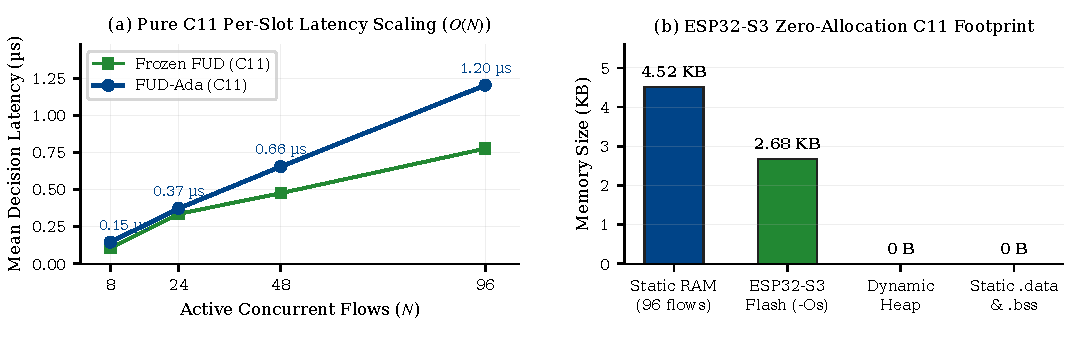
\includegraphics[width=\textwidth]{figures/fig05_c11_scaling.pdf}
\caption{Zero-allocation pure C11 gateway scheduler benchmark under on-chip ESP32-S3 execution (240\,MHz Xtensa LX7, \texttt{-Os}): (a) measured on-chip per-slot latency scaling ($O(N)$) across $N \in \{8, 24, 48, 96\}$ flows (500 steady-state iterations/point via \texttt{esp\_timer\_get\_time()}); (b) static RAM, flash \texttt{.text}, and hardware-verified 0~B runtime heap delta.}
\label{fig:c11}
\end{figure*}

\begin{table}[!t]
\centering
\caption{Zero-Allocation Pure C11 Kernel Footprint and On-Chip ESP32-S3 Benchmark}
\label{tab:c11}
\scriptsize
\setlength{\tabcolsep}{1.0pt}
\begin{tabular}{@{}lc@{}}
\toprule
Metric (\texttt{-std=c11 -Wall -Wextra -Werror}) & Measured Value \\
\midrule
Static RAM (\texttt{na\_sched\_t}, 96 flows) & \textbf{4,624~B} (4.52\,KB, 0.88\% SRAM) \\
ESP32-S3 \texttt{-Os} flash (8 policies) & \textbf{2,746~B} (2.68\,KB \texttt{.text}) \\
ESP32-S3 static \texttt{.data} / \texttt{.bss} & \textbf{0~B} / \textbf{0~B} \\
ESP32-S3 runtime heap delta (on-chip) & \textbf{0~B} (361,620~B unchanged) \\
ESP32-S3 \texttt{FUD-Ada} ($N{=}8/24/48/96$) & \textbf{0.20 / 0.67 / 1.39 / 2.91\,ms} \\
ESP32-S3 \texttt{FUD-Quad} ($N{=}8/24/48/96$) & 0.13 / 0.36 / 0.68 / 1.32\,ms \\
Host arm64 \texttt{FUD-Ada} ($N{=}8/24/48/96$) & 0.15 / 0.37 / 0.66 / 1.20\,$\mu$s \\
Python--C11 parity ($<10^{-11}$) & \textbf{24 / 24} full trajectories \\
\bottomrule
\end{tabular}
\end{table}

\section{Discussion, Operational Regimes, and Limitations}

Our multi-cohort evidence clarifies exact operational choices for IoT gateway designers:
\begin{itemize}
\item \textbf{General-Purpose Congested, Bursty, and Lossy Gateways:} \texttt{FUD-Ada} delivers the lowest event deadline miss among all 14 comparators under Congestion, Bursty, and measured E220 hardware loss logs without suffering the catastrophic state-AoI starvation of \texttt{EDF} (12.7--53.1\,s), \texttt{MaxWeight} (61.6--103.2\,s), or \texttt{Priority} (103.7--121.3\,s).
\item \textbf{Cross-Regime Comparison Against \texttt{AoI-Gain}:} While \texttt{AoI-Gain} is competitive in isolation on highly asynchronous bursts (statistically tied on Intel Berkeley event miss, $p_{\text{Holm}}{=}0.927$), its performance degrades substantially under periodic congestion (+9.91\,pp miss), 4$\times$ bursts (+7.27\,pp miss), and measured E220 loss logs (+5.62\,pp miss); \texttt{FUD-Ada} therefore offers the strongest cross-regime robustness for general IoT gateways.
\item \textbf{Equal-Share Throughput Only:} \texttt{PF} achieves near-1.0 raw Jain but misses 69--79\% of critical events.
\end{itemize}

\paragraph{Explicit Scope Limitations}
Two practical boundaries remain open for future work. First, while Study~II performs trace-driven replay over measured ESP32-S3 + E220 hardware loss logs, Study~III uses real 54-mote arrival timestamps, and Section~V-D measures direct on-chip ESP32-S3 execution cycles and zero-heap execution, live multi-node RF medium-access contention (CSMA/ALOHA collisions across dozens of physical radios) and oscilloscope-measured board power/battery lifetime remain unmeasured. Second, Study~III maps 4 real hours of indoor mote arrivals into 4,000 gateway slots to create controlled gateway saturation; field deployment timings will depend on exact radio spreading factors and regional duty-cycle laws. Single-precision \texttt{float} acceleration on Xtensa LX7's hardware FPU can further cut ESP32-S3 execution time by $>5\times$ when strict $<10^{-11}$ Python parity is relaxed.

\section{Conclusion}
We diagnosed and resolved the quadratic-AoI and unscaled-debt mismatch in multi-flow IoT gateway scheduling through \texttt{FUD-Ada}, a scale-matched $O(N)$ scheduler combining square-root state freshness, deadline-feasible urgency, and Lyapunov logarithmic debt with proved scale bounds and asymptotic starvation-freedom. Across 17,820 total runs (including 5,340 new held-out runs spanning synthetic stress, trace-driven replay over 24 measured ESP32-S3 + E220 Sub-GHz hardware loss logs, and 12 held-out days of 54-mote MIT Intel Berkeley traffic), \texttt{FUD-Ada} achieves Holm-significant event-miss reductions over classical baselines (FIFO, RR/WRR, EDF, MaxWeight, PF, \texttt{AoI-Gain}, and \texttt{FUD-Quad}), strictly Pareto-dominates EDF on real 54-mote traffic, resolves the debt-fairness ablation across all cohorts, and executes directly on ESP32-S3 silicon (240\,MHz) in 0.20--2.91\,ms/slot, 4.52\,KB static RAM, 2.68\,KB flash, and 0~B runtime heap delta.

\bibliographystyle{IEEEtran}
\bibliography{references}

\end{document}
